
\documentclass[../mcmpaper]{subfiles}
\begin{document}
	\section{Model 1: LDA Topic Extraction and Data Analysis}
	
	\subsection{Data Preprocessing}
    Since there are no vacant values in the data file, they can be ignored.Other data processing, such as data standardization and feature coding, will be mentioned in the specific model. Below, only abnormal data will be judged and processed.
    \par
    For each sample comment, marketplace, product\_id, and other irrelevant attributes can be deleted. Verified\_purchase for Y indicates that the customer has purchased the product for close to the original price, and Vine for Y indicates that the customer has gained trust in the Amazon community due to the accuracy and insight of the review.Vine members are trustworthy, but we are suspicious of non-Vine members.Comments with Vine N and verified\_purchase N lack credibility if the reviewer is not a Vine member and did not purchase the product at close to its original price or at all (since reviews may lack authenticity if they are heavily discounted).Table~\ref{tab:4.1.1} gives an example of an untrustworthy review that exists in all three data sets.\\[1em]
    \begin{minipage}{1.0\linewidth}
    \captionof{table}{Examples of untrustworthy comments}
    \label{tab:4.1.1}
    \begin{tblr}{
          width=\linewidth,
          colspec={*{6}{X[c]}},
          hline{1, Z} = {2pt, solid},
          hline{2} = {solid}
        }
        marketplace & customer\_id & … & vine & verified\_purchase & …  & review\_date \\
        US & 39431051 & … & N & N & … & 8/31/2015\\
    \end{tblr}
    \end{minipage}
    \subsection{Data Visualization}
    Since the actual situation of the possible data of the three products was different, we visualized the three products and analyzed the results respectively.First, visualize the review stars, as shown in Figure~\ref{fig:4.2.1}.
    \begin{figure}[!ht]
    \centering
    \subfigure[pacifier\_star\_ratio]{
       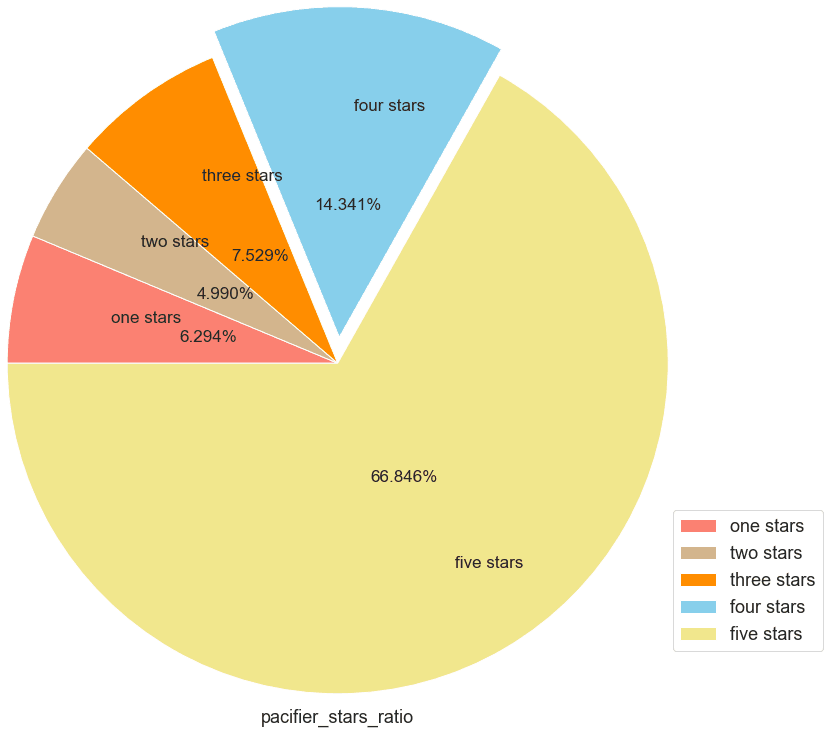
\includegraphics[scale=0.12]{4.2.1}
    }
    \qquad
	\subfigure[hair\_dryer\_star\_ratio]{
      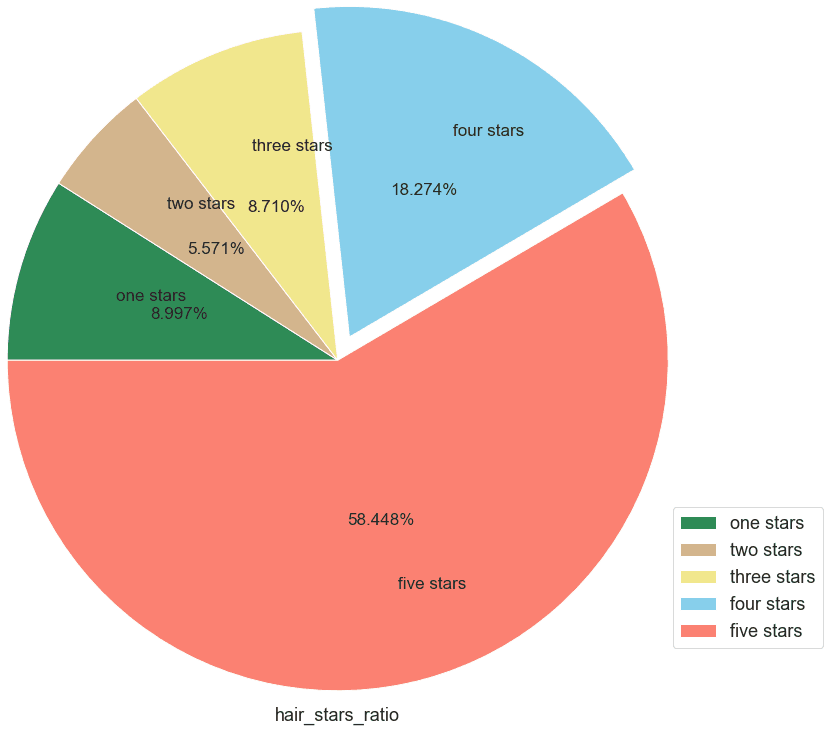
\includegraphics[scale=0.12]{4.2.2}
    }
    \qquad
    \subfigure[microwave\_star\_ratio]{
      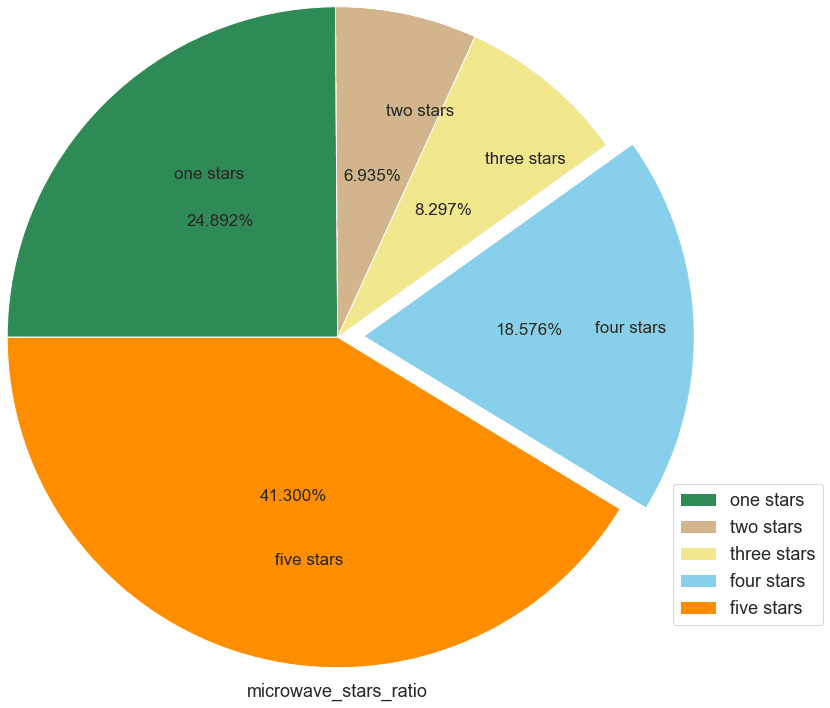
\includegraphics[scale=0.12]{4.2.3}
    }
    \captionof{figure}{The proportion of five stars in the star\_rating of each product}
    \label{fig:4.2.1}
    \end{figure}
    \par
    It can be seen from Figure~\ref{fig:4.2.1} that five-star reviews are always the most among the three products. The star distribution of pacifier and Hair\_dryer is roughly the same, while the two-star reviews are the least, indicating that the quality of the two products is generally satisfactory, but it still needs to be strengthened.However, one-star reviews in microwave are close to 24.892\%, second only to five-star reviews, indicating that there may be quality problems and other aspects, and the specific content of one-star reviews should be paid attention to.
    \par
    To take advantage of comments' useful voting, we define a variable that measures how helpful a comment is: $helpful\_Ratio$, which represents the likelihood that the comment will be helpful.Intuitively, the expression of help rate is $helpful\_votes/total\_votes$, but considering that $total_votes$ cannot be calculated when it is 0, and comments cannot simply be considered to be unhelpful, \textbf{sigmoid} function $y=\frac{1}{1+e^{x}}$ is used to solve this problem.The sigmoid function image is shown in Figure~\ref{fig:4.2.4}.\\[1em]
    \begin{minipage}{1.0\linewidth}
    \centering
    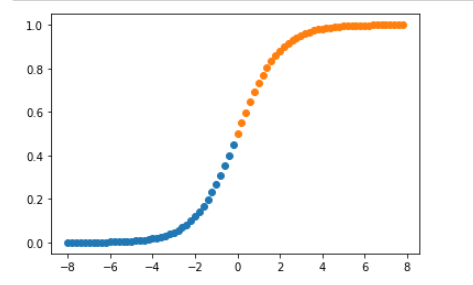
\includegraphics[scale=0.5]{4.2.4}
    \captionof{figure}{Image of sigmoid function}
    \label{fig:4.2.4}
    \end{minipage}
    \par
   Make helpful\_ratio=$y$,,$x$=helpful\_votes-(total\_votes-helpful\_votes), and you get .After calculation, the helpful\_ratio is greater than 0.5 as helpful comments, less than 0.5 as unhelpful comments, equal to 0.5 not sure whether helpful.Figure~\ref{fig:4.2.5} shows the large distribution of helpful comments.\\[1em]
    \begin{minipage}{1.0\linewidth}
    \centering
    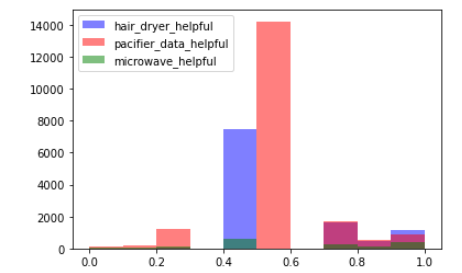
\includegraphics[scale=0.5]{4.2.5}
    \captionof{figure}{Distribution of helpful comments}
    \label{fig:4.2.5}
    \end{minipage}
    \par
    It can be found from Figure~\ref{fig:4.2.5} that most of the help rates of pacifier and hair\_dryer are concentrated around 0.5, and the help rate is basically not too low. As the microwave data volume only has 1432 comments after data cleaning, basically at 0.5 and 0.8-1.0, indicating that there are many helpful comments.
    \subsection{Descriptive Statistics}
    The following describes the statistics of stars and helpful\_ratio. Microwave is taken as an example.
    \begin{figure}[!ht]
    \centering
    \begin{minipage}[b]{0.45\linewidth}
    	\captionof{table}{Star description statistics}
        \label{tab:4.3.1}
        \begin{tblr}{
              width=\linewidth,
              colspec={X[c]X[c]},
              hline{1, Z} = {2pt, solid},
              hline{2} = {solid}
            }
            Statistics & Numerical value\\
            mean & 3.45\\
            std & 1.65\\
            min & 1\\
            25th percentile & 1\\
            50th percentile & 4\\
            75th percentile & 5\\
            max & 5
        \end{tblr}
        \end{minipage}
        \qquad
        \begin{minipage}[b]{0.45\linewidth}
    	\captionof{table}{Helpful\_ratio Description statistics}
        \label{tab:4.3.2}
        \begin{tblr}{
              width=\linewidth,
              colspec={X[c]X[c]},
              hline{1, Z} = {2pt, solid},
              hline{2} = {solid}
            }
            Statistics & Numerical value\\
            mean & 0.72\\
            std & 0.21\\
            min & 0.5\\
            25th percentile & 0.5\\
            50th percentile & 0.73\\
            75th percentile & 0.95\\
            max & 1
        \end{tblr}
    \end{minipage}
    \end{figure}
    It can be seen from Table~\ref{tab:4.3.1} that the star rating is between 1 and 5, divided into 5 levels, with an average value of 3.45, indicating that the average microwave star rating is between 3 and 4, and microwave evaluation can be considered as general only by the star rating. Table~\ref{tab:4.3.2} shows that the mean helpful\_ratio of Microwave is 0.72, and the score is 0.5-1, indicating that the data cleaning effect is very good, and there are almost no comments with a help rate lower than 0.5.
    \subsection{Topic Extraction Model Based on LDA}
    \paragraph{Model Construction}
    Latent Dirichlet Allocation(LDA)\cite{1} topic model proposed by Blei in 2003, is a three-layer Bayesian probability model extended on the probabilistic implicit semantic index (pLSI), is a document generation probability model.The LDA model consists of three layers: term, topic and document. The basic idea is to treat a document as a mixture of its implied topics.Documents to topics follow a polynomial distribution, and topics to words follow a polynomial distribution.The purpose is to identify topics, that is, the document vocabulary matrix is divided into document topic matrix and topic vocabulary matrix.LDA\cite{2} has had a huge impact in the field of natural language processing and statistical machine learning, and has quickly become one of the most popular probabilistic text modeling techniques in machine learning.
    \par
    Suppose in the document set, the number of documents is A, the number of words in the document is B, and there are C topics in the document set. $\beta_i$ represents the i-th topic, $\zeta_i$ represents the topic distribution of document J, $W_{j,z}$ and $Z_{i, j}$ represent the n-th word in document J and its topic respectively, $\eta$ and $\alpha$ represent the hyperparameter of topic distribution and the hyperparameter of document topic distribution respectively.Figure~\ref{fig:4.4.1} shows the graphical structure of the LDA model.
    \begin{figure}[!ht]
    \centering
    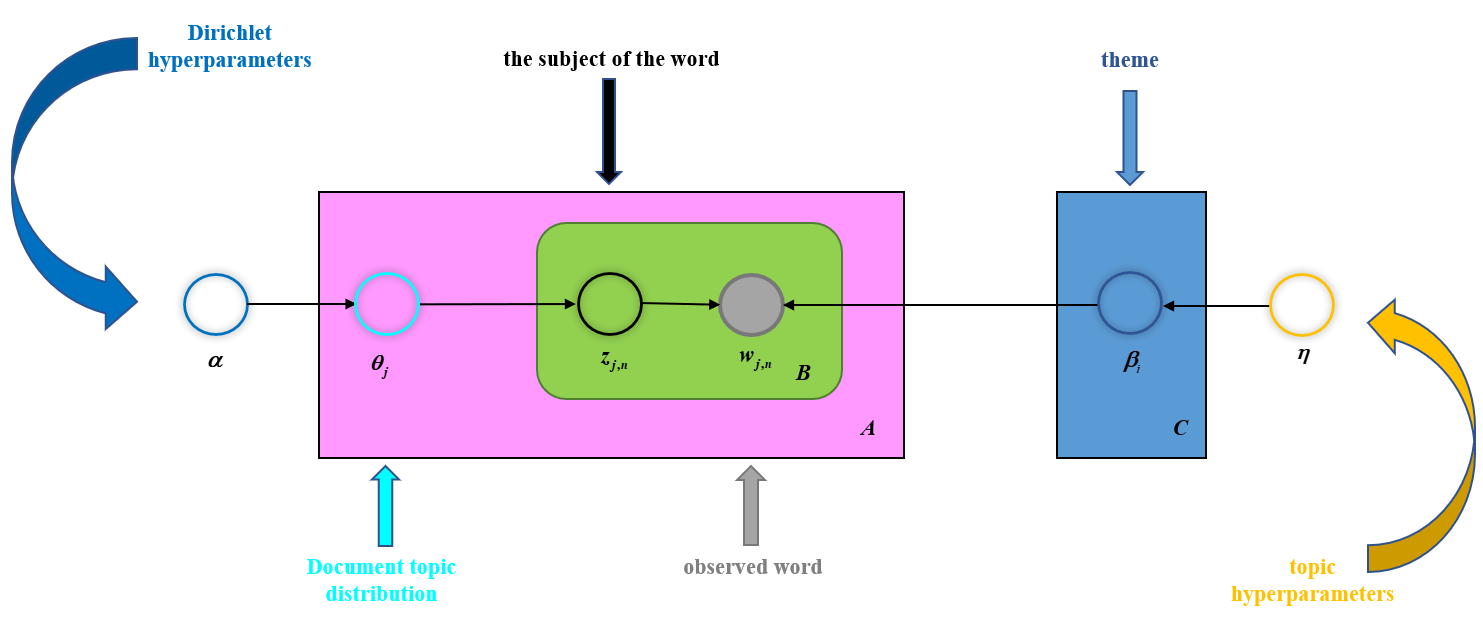
\includegraphics[scale=0.3]{4.4.1}
    \captionof{figure}{Graphical structure of LDA model}
    \label{fig:4.4.1}
    \end{figure}
    \par
    The joint probability density of implied variables and observed variables in the LDA model is:
    \begin{equation}
    \begin{aligned}
    p(\theta, \beta, w, z \mid \eta, a) &=p(\theta \mid \alpha) p(\beta \mid \eta) p(w \mid \beta, z) p(z \mid \theta) \\
    &=\prod_{-1}^{D} p\left(\theta_{j} \mid \alpha\right) \prod_{\zeta=1}^{c} p\left(\beta_{1} \mid \eta\right) \prod_{n=1} p\left(w_{1, n} \mid z_{j, n}, \beta_{z}\right) p\left(z_{j, n} \mid \theta_{j}\right.
    \end{aligned}
    \end{equation}
    Among them, subject to dirichlet distribution has $P(\Theta_i|\alpha)$ and $P(\beta_i|\eta)$, but $P(w_{j,n}|z(j, n), \beta_{i, n})$ and $P(z_{j,n}|\Theta_j)$ obey the multinomial distribution.
    \par
    Variational reasoning and Gibbs sampling are usually used for parameter estimation of LDA model.Both are approximate estimation methods, each has its own advantages and disadvantages, depending on the situation to choose appropriate methods.In general, Gibbs sampling is easy to realize but inefficient, while variational reasoning is complicated but efficient.
    \paragraph{Results and Analysis}
    Based on the LDA topic analysis algorithm, we extracted the subject words of the comments, used the wordcloud library of python to display the wordcloud, and gave an explanation.
    \par
    As can be seen from the Figure~\ref{fig:4.4.a}, most of the customer comments on the three products are positive, with Fivestars accounting for a large proportion. From the word cloud, it can be seen that the favorable comments mainly contain words such as love, great, cute and nice, while the negative comments are related to words such as problem, broke and problem.
    \begin{figure}[!ht]
    \centering
    \subfigure[Wordcloud of pacifier]{
      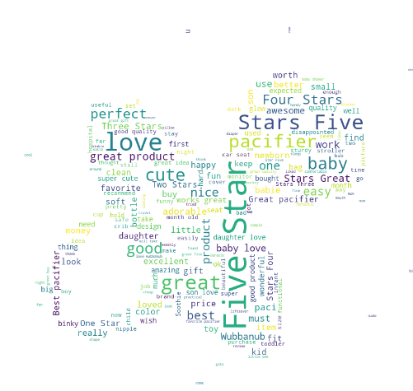
\includegraphics[scale=0.8]{4.4.2}
    }
    \subfigure[Wordcloud of hair\_dryer]{
      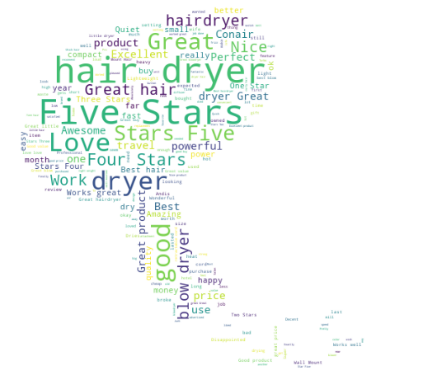
\includegraphics[scale=0.8]{4.4.3}
    }
    \subfigure[Wordcloud of microwave]{
      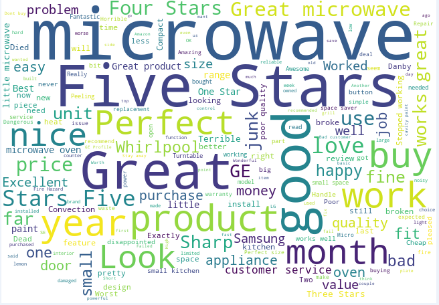
\includegraphics[scale=0.8]{4.4.4}
    }
    \caption{Subject word cloud extracted by LDA}
    \label{fig:4.4.a}
    \end{figure}
   
    \section{Model 2: Screening Valuable Reviews Based on K-Means And Word2vec}
    \subsection{Model Construction}
    First, we have used LDA to get the topic of each valid comment. Next, we use the self-built corpus of comments to construct 5 classic example sentences, and the corresponding scores are 0.1, 0.3, 0.5, 0.7 and 0.9. Similarity analysis is conducted between all valid comments and these 5 classic example sentences.The score of each comment is the product of the score of the classic example with the greatest similarity and the maximum similarity. We call the score satisfaction rate and mark it as S.
	\paragraph{Word2vec Algorithm}
    Word2vec\cite{3} is an implementation of the model proposed by Mikolov et al. It can train word vector quickly and effectively.It contains two training models, CBOW and Skip\_gram respectively, and their schematic diagrams are shown in FIG~\ref{fig:5.1.1} and \ref{fig:5.1.1}.
    \begin{figure}[!ht]
    \centering
    \subfigure[Wordcloud of pacifier]{
      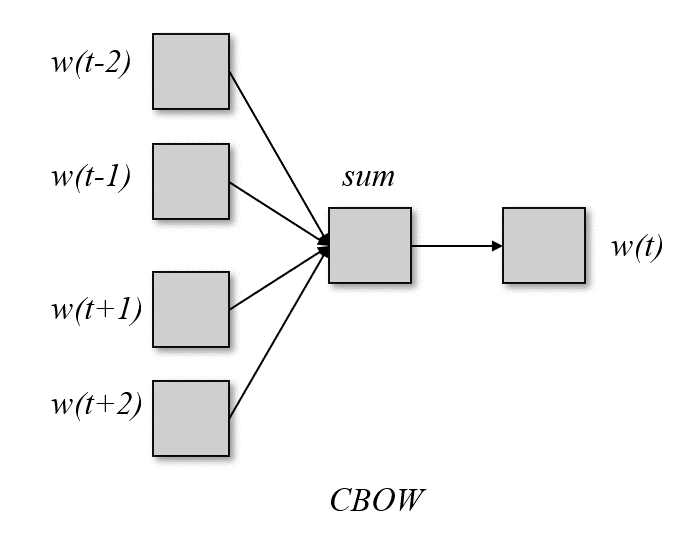
\includegraphics[scale=0.35]{5.1.1}
      \label{fig:5.1.1}
    }
    \subfigure[Wordcloud of hair\_dryer]{
      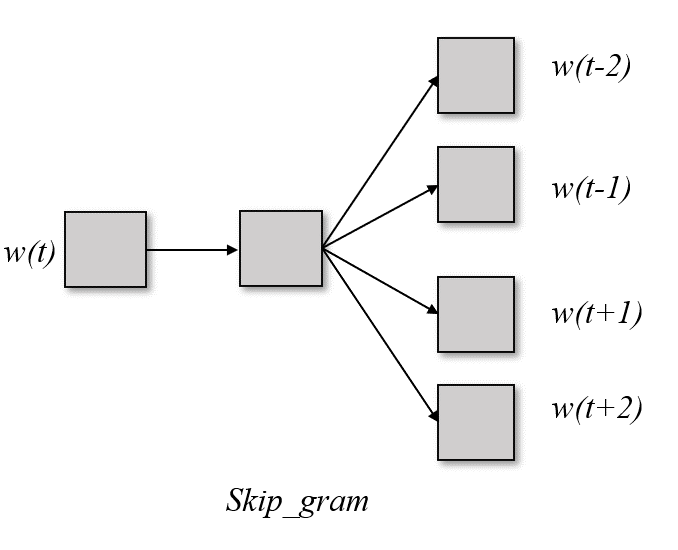
\includegraphics[scale=0.35]{5.1.2}
      \label{fig:5.1.2}
    }
    \caption{CBOW and Skip\_gram structure framework}
    \label{fig:5.1.a}
    \end{figure}
    It can be seen from Figure~\ref{fig:5.1.a} that both models have three layers, namely, input, hidden and output layers.If a word is used as input to predict the context, then the model is called Skip-Gram model; if the context of a word is used as input to predict the word itself, then it is the CBOW model.\\[1em]
    \begin{minipage}{1.0\linewidth}
    \captionof{table}{word2vec word vector training framework}
    \label{tab:5.1.1}
    \begin{tblr}{
          width=\linewidth,
          colspec={*{3}{X[c]}},
          hline{1, Z} = {2pt, solid},
          hline{2} = {solid}
        }
        model & CBOW & Skip\_gram\\
        Hierachy Softmax & CBOW+HS & Skip\_gram+HS\\
        Negative Sampling & CBOW+NS & Skip\_gram+NS
    \end{tblr}
    \end{minipage}
    \par
    Table~\ref{tab:5.1.1} shows two optimization methods of Word2VEc to improve training efficiency and four word vector training frameworks combined with two training models.
	\paragraph{K-Means Clustering Algorithm}
    K-means\cite{4} algorithm is an unsupervised learning and clustering algorithm based on partition. Generally, Euclidean distance is used as an indicator to measure the similarity between data objects. The similarity is inversely proportional to the distance between data objects, and the larger the similarity, the smaller the distance.Figure~\ref{fig:5.2.1} is the k-means algorithm flow chart. We perform K-means clustering according to satisfaction, Helpful\_ratio and star rating.\\[1em]
    \begin{minipage}{1.0\linewidth}
    \centering
    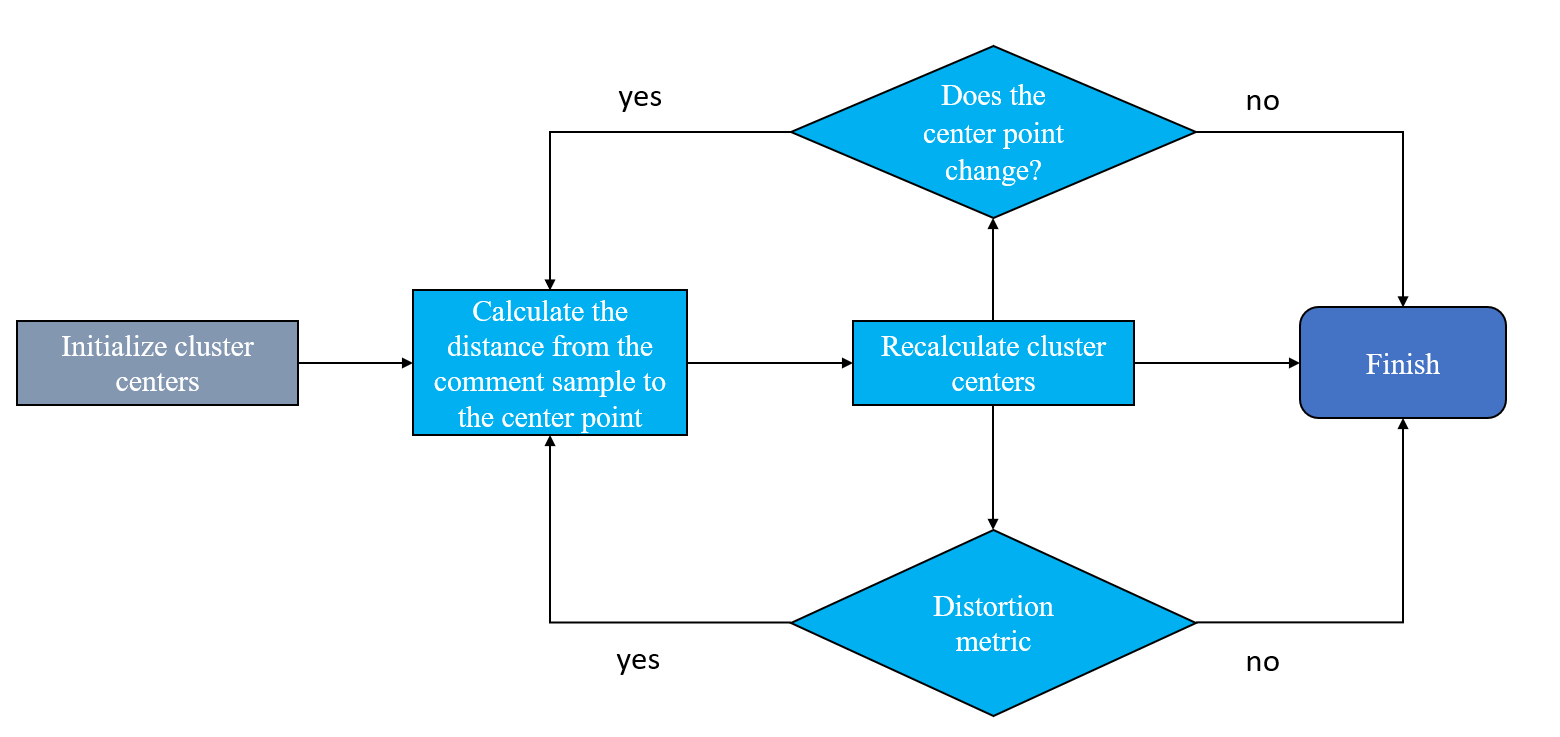
\includegraphics[scale=0.3]{5.2.1}
    \captionof{figure}{K-means flow chart}
    \label{fig:5.2.1}
    \end{minipage}
    \subsection{Results and Analysis}
    The following analysis only takes Hair\_Dryer as an example, and the analysis of other two products is similar.Table~\ref{tab:5.2.1} shows satisfaction rates for some of the comments.\\[1em]
    \begin{minipage}{1.0\linewidth}
    \captionof{table}{Satisfaction rate for some reviews of hair\_dryer}
    \label{tab:5.2.1}
    \begin{tblr}{
          width=\linewidth,
          colspec={*{5}{X[c]}},
          hline{1, Z} = {2pt, solid},
          hline{2} = {solid}
        }
        marketplace & customer\_id & review\_id & & S\\
        US & 51995766 & R230LCPQDOFJJZ & … & 0.87\\
        US & 39431051 & R21NN9ONVZITI0 & … & 0.79\\
        … & … & … & … & …\\
        US & 9924936 & R3N0F2FKJOMGKK & … &0.95\\
    \end{tblr}
    \end{minipage}
    \par
    Then, satisfaction, Helpful\_ratio and stars are used for K-means clustering. The number of clusters is set to 4, and the given numbers 1,2,3 and 4 respectively represent very good, good, poor and very poor.Sort out the clustering results, add category numbers to the data shown in Table 5, and show the clustering effect of satisfaction, Helpful\_ratio and star rating together, as shown in Table~\ref{tab:5.2.2}.\\[1em]
    \begin{minipage}{1.0\linewidth}
    \captionof{table}{some reviews of hair\_dryer}
    \label{tab:5.2.2}
    \begin{tblr}{
          width=\linewidth,
          colspec={*{6}{X[c]}},
          hline{1, Z} = {2pt, solid},
          hline{2} = {solid}
        }
        review\_id & … & star\_rating & helpful\_ratio & S &category\\
        R230LCPQDOFJJZ & … & 5 & 0.5 & 0.87 & 2\\
        R21NN9ONVZITI0 & … & 1 & 0.5 & 0.79 & 4\\
        … & … & … & … & …\\
        R3N0F2FKJOMGKK & … & 5 & 0.95 & 0.95 & 1
    \end{tblr}
    \end{minipage}
    \par
    It is not difficult to find from Table~\ref{tab:5.2.2} that reviews with low star rating and low helpful\_ratio are usually in category 3 and 4, that is, "poor" and "very poor" reviews, indicating that customers are dissatisfied with the product and give comments on business trips; while reviews with high star rating and high helpful\_ratio are basically in category 1 and 2, indicating that customers are satisfied with the product and give favorable comments.Similarly, reviews in category 2 tend to be favorable, which we define as "good", and reviews in category 3 tend to be negative, which we define as "poor".This is consistent with the actual situation, which shows that the calculation of model and satisfaction rate is reasonable.
    \section{Reputation Prediction Based on EWM-TOPSIS and ARIMA}
    \subsection{Model Construction}
    \paragraph{EWM-TOPSIS Algorithm}
    According to the requirements of the title, we need to find time-based measures and patterns to reflect the increase or decrease of product reputation, so we need to define reputation rate R, which is constructed by EWM-Topsis algorithm, that is, R is the comprehensive score, and then we need to use time series model ARIMA to predict reputation.
    \par
    TOPSIS\cite{5} is a comprehensive evaluation method to determine the advantages and disadvantages of evaluation objects. It makes full use of known initial data information and the results can well reflect the differences between evaluation schemes, which is widely applied in many fields.Considering that the weight coefficients of each index may not be equal, entropy weight method (EWM) is introduced to determine the weight, which is more objective than AHP.
    \paragraph{The steps of ewM-TopSIS model construction in this paper are as follows:}
    \subparagraph{1} Construct decision matrix A. Since there are three indicators including satisfaction, help rate and star rating, m=3 and n depends on specific products.
    \begin{equation}
    \mathrm{A}=\left[\begin{array}{cccc}
    a_{11} & a_{12} & \ldots & a_{1 m} \\
    a_{21} & a_{22} & \ldots & a_{2 m} \\
    \vdots & \vdots & \ddots & \vdots \\
    a_{n 1} & a_{n 2} & \ldots & a_{n n}
    \end{array}\right]
    \end{equation}
    \subparagraph{2} The decision matrix index is forward.The extremely small, intermediate and interval indicators are transformed into extremely large indicators, which do not need to be transformed because they are all extremely large indicators.
    \subparagraph{3} standardize the decision matrix, set the standardized matrix as B, and each element in B:
    \begin{equation}
    b_{1 j}=\frac{1}{a_{i j}}\sqrt{\sum_{i=1}^{n} a_{i j}}
    \end{equation}
    \par
    If there is A negative number in matrix A, the Min-Max normalization method is used:
    \begin{equation}
    b_{i j}=\frac{a_{i j}-\min \left\{x_{1}, \ldots, x_{\pi j}\right\}}{\max \left\{x_{1}, \ldots, x_{\pi j}\right\}-\min \left\{x_{1}, \ldots, x_{\pi y}\right\}}
    \end{equation}
    \subparagraph{4}
    The index weight is determined based on EWM method, and the non-negative matrix is obtained by \textbf{Step 3}, and the probability matrix P is calculated, where the value of each element is:
    \begin{equation}
    p_{n j}=\frac{b_{i j}}{\sum_{i=1}^{n} b_{i j}}
    \end{equation}
    and $\sum_{i=1}^{n}b_{i,j}=1$. Then calculate the information entropy of the j-th indicator $E_j$:
    \begin{equation}
    E_{j}=-\frac{1}{\operatorname{In}(n)} \sum_{-1}^{n} p_{1 j} \operatorname{In}\left(p_{i j}\right)
    \end{equation}
    then calculate the information utility $V_j$:
    \begin{equation}
    V_j=1-E_{j}
    \end{equation}
    Finally, the weight of each index is obtained by normalization $W_j$:
    \begin{equation}
    W=\frac{V_{j}}{\sum_{j=1}^{m} V_{j}}(\mathrm{j}=1,2, \ldots, \mathrm{m})
    \end{equation}
    \subparagraph{5}
    Calculate the score and normalize the treatment.Define maximum value $\mathrm{A}+{}$ and minimum value $\mathrm{B}-$:
    \begin{equation}
    \begin{aligned}
    &B^{-}=\left(B_{1}^{-}, B_{2}^{+}, \ldots, B_{m}^{+}\right)=\left(\max \left\{b_{11}, b_{21}, \ldots, b_{n 1}\right\}, \ldots, \max \left\{b_{1 m}, b_{2 \pi}, \ldots, b_{n m}\right\}\right) \\
    &B^{-}=\left(B_{1}^{-}, B_{2}^{-}, \ldots, B_{m}^{-}\right)=\left(\min \left\{b_{11}, b_{21}, \ldots, b_{n 1}\right\}, \ldots, \min \left\{b_{1 m}, b_{2 m}, \ldots, b_{n m}\right\}\right)
    \end{aligned}
    \end{equation}
    at the same time define the distance between the ith comment object and the maximum value $\mathrm{D_i}+$ and the minimum value $\mathrm{D_i}-$ as follows:
    \begin{equation}
    D_{i}^{*}=\sqrt{\sum_{-1}^{m} W_{j}\left(b_{i j}-B_{j}^{+}\right)^{2}}, \quad D_{i}^{-}=\sqrt{\sum_{-1}^{m} W_{j}\left(b_{i j}-B_{j}^{-}\right)^{2}}
    \end{equation}
    Then the unnormalized score of the ith comment object $S_i$ calculated as:
    \begin{equation}
    S_{i}=\frac{D_{1}^{-}}{D_{i}^{+}+D_{i}^{-}}
    \end{equation}
    Finally, the normalization can obtain $S_{1}=S_{1} / \sum_{i=1}^{n} S_{1}$ represents the final score of the i-th comment.
    \paragraph{ARIMA Time Series Analysis}
    ARIMA model, short for autoregrestive moving average model, is a famous time series prediction method proposed by Box and Jenkins in the early 1970s\cite{7}. ARIMA(p,d,q), p represents the order of autoregression, d represents the order of difference, and q represents the order of moving average.The model can be expressed as:
    \begin{equation}
    \left(1-\sum_{i=1}^{p} \phi_{i} L^{i}\right)(1-L)^{d} X_{t}=\left(1+\sum_{i=1}^{q} \theta_{i} L^{i}\right) \varepsilon_{t}
    \end{equation}
    L is a lag operator and d is a positive integer.
    \par
    The difference expression is as follows:
    \begin{equation}
    \left\{\begin{array}{l}
    \phi(B) \nabla^{d} X_{t}=\theta(B) \varepsilon_{t}, \\
    E\left(\varepsilon_{t}\right)=0, \operatorname{Var}\left(\varepsilon_{t}\right)=\sigma^{2}, E\left(\varepsilon_{t} \varepsilon_{s}\right)=0, S \neq 1, \\
    E\left(X_{s} X_{t}\right)=0, \nabla S<t .
    \end{array}\right.
    \end{equation}
    Time series model can be transformed into stationary time series model by difference operation.
    \par
    \begin{equation}
    \nabla^{d}X_1=\sum_{i=1}^{d}(-1)^{d} C_{d}^{i} X_{t-1} \text {,among them, } C_{d}^{j}=\frac{d !}{i !(d-i) !}
    \end{equation}
    For $d$ in the model, when $d=0$, ARIMA(p,d,q) model is actually ARIMA(p,q) model; When $p=0$, ARIMA(p,d,q) model is denoted as IMA(p,d); When $q=0$, ARIMA(p,d,q) model is simply denoted as ARI(p,d).When d=1,p=q=0, ARIMA(p,d,q) model is called random walk model, namely:
    \subsection{Results and Analysis}
    After the program is run, the reputation rates of pacifier, hair\_dryer and microwave are obtained respectively. We only take pacifier as an example, and the results obtained are shown in Table\ref{tab:5.2.1}.\\[1em]
    \begin{minipage}{1.0\linewidth}
    \captionof{table}{Reputation rate for pacifier data}
    \label{tab:6.2.1}
    \begin{tblr}{
          width=\linewidth,
          colspec={*{5}{X[c]}},
          hline{1, Z} = {2pt, solid},
          hline{2} = {solid}
        }
        marketplace & customer\_id & review\_id &  & R\\
        US & 40626522 & R1A3ZUBR8TSAKY & … & 0.00006046\\
        US & 15312194 & RG9XY3EKPUCL1 & … & 0.00003773\\
        … & … & … & … & … \\
        US & 20849759 & rzhlaecz5ztnc & … & 0\\
    \end{tblr}
    \end{minipage}
    \par
    It can be seen from the three tables that R is small because of the large amount of data, which will result in a small R after normalization.Even after data pretreatment, there will still be comments with a reputation rate of 0, which indicates that it is not reliable to only look at the star rating, but also refer to the satisfaction rate and help rate.
    \par
    Next, SPSS's expert modeler was used for time series analysis, as shown in Figure~\ref{fig:6.2.1.a}.
    \begin{figure}[!ht]
    \centering
    \subfigure[ACF and PACF]{
      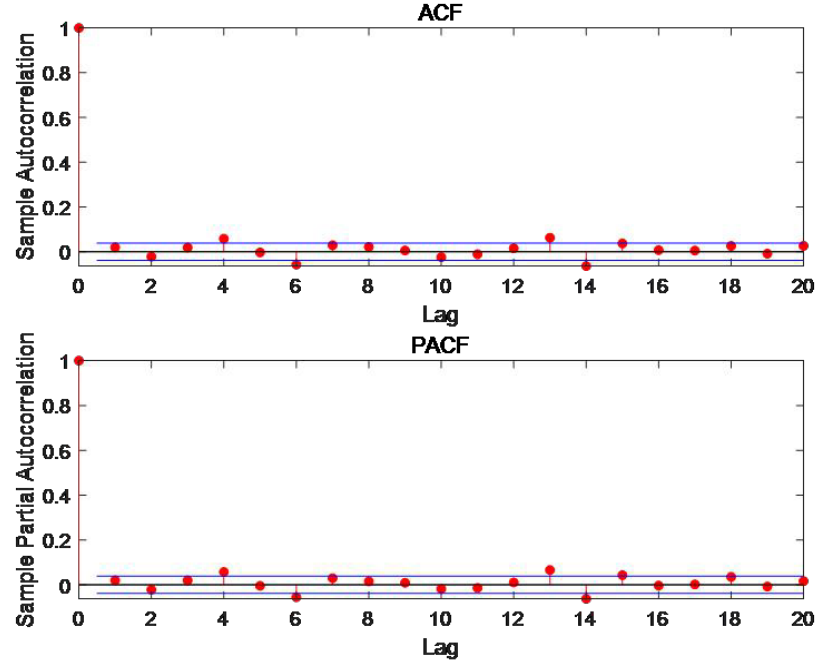
\includegraphics[scale=0.3]{6.2.1}
      \label{fig:6.2.1}
    }
    \qquad
	\subfigure[Sequence diagram and prediction results]{
      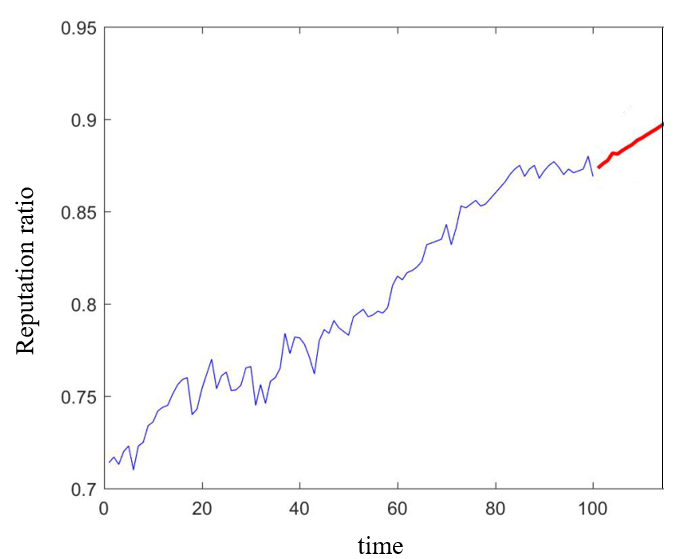
\includegraphics[scale=0.35]{6.2.2}
      \label{fig:6.2.2}
    }
    \captionof{figure}{Time series analysis of a single comment sample}
    \label{fig:6.2.1.a}
    \end{figure}
    In order to show the increasing and decreasing trend of comment reputation rate, we selected the comment with product\_ID B013RF851A from pacifier dataset as an example.It can be seen from FIG~\ref{fig:6.2.2} that the reputation rate of this review keeps increasing trend, which requires differential processing. The first-order difference is determined by testing and significance test, that is, d =1. From the ACF and PACF images in FIG~\ref{fig:6.2.1}, it can be found that both are trailing.So the model is ARIMA(3,1,3).FIG~\ref{fig:6.2.2} also shows that the reputation rate of the sample review has an increasing trend.
    \section{Product Classification Model Based on SVM}
    \subsection{Model Construction}
    Since the division of failed products and successful products is not clear, we need to use existing data and reputation rate to establish a SVM model. In order to facilitate the following description, we name the products as normal products and abnormal products, and use SVM to identify potential successful or failed products.
    \par
    SVM\cite{6} in the SLT (StatisticalLearningTheory) based on a machine learning method, has been widely used in pattern classification, function estimation, regression analysis and other fields.It contains three ideas: optimal hyperplane technique, soft interval and inner product kernel function.
    \paragraph{The SVM Classifier}
    For the dichotomous problem, SVM separates two different classes by training a hyperplane, namely successful products and failed products in this problem.Assuming that the hyperplane can accurately classify training samples, the hyperplane can be described by the following equation:
    \begin{equation}
    W^TX+b=0
    \end{equation}
    Where $W=(W_1, W_2,\dots,W_d)$ represents the normal vector, $b$ represents the displacement term, and the partition of the hyperplane is determined by $W$ and $b$. Give the training set $D=\{(x_1, y_1),(x_2, y_2),\dots,(x_m, y_m),y_i\in \{+1, -1\}\}$, For $(x_i,y_i)\in D$, there are:
    \begin{equation}
    \left\{\begin{array}{l}
    w^{T} x+b \geq+1, y_{1}=+1 \\
    w^{\top} x+b \leq-1, y_{1}=-1
    \end{array}\right.
    \end{equation}
    We define a product as a successful product $y_i=+1$ and a failed product $y_i=-1$.We hope to find some of the largest interval partitioning hyperplane, which under the constraints problem:
    \begin{equation}
    \begin{aligned}
    &\min _{w ; b} \frac{1}{2}\|w\|^{2} \\
    &st.\left(x_{i}+b\right) \geq 1, i=1,2, \ldots, m .
    \end{aligned}
    \end{equation}
    Usually uses dual problem solving and SMO methods to deal with dual problems. If some sample division errors can be allowed, "soft interval" is used to introduce relaxation variable solution.
    \paragraph{One Class SVM}
    Since the conditions for judging successful or failed products are not given in this paper, OneClassSVM needs to be introduced to distinguish successful products from failed products. The goal of OneClassSVM is to separate data points from the origin as much as possible in the feature graph space. Firstly, the data points are projected onto the feature space using gaussian kernel, and then the quadratic programming problem is solved to separate the projected data points from the origin.
    \subsection{Results and Analysis}
    OneClassSVM was first used to determine outliers of reputation rates that represent the presence of potentially successful or failed products.LSVM is then trained using OneClassSVM as a potential success or failure threshold for the product.Taking the Pacifier data set as an example, we found the corresponding successful products and failed products.Partial results are shown in Table~\ref{tab:7.2.1}:\\[1em]
    \begin{minipage}{1.0\linewidth}
    \captionof{table}{Potentially successful or failing products}
    \label{tab:7.2.1}
    \begin{tblr}{
          width=\linewidth,
          colspec={*{5}{X[c]}},
          hline{1, Z} = {2pt, solid},
          hline{2} = {solid}
        }
        product\_id & b00f8nkkzo & B003CK3LDI & B00B7U61RI & b00hnjo5uw\\
        Classification result & success & fail & success & fail\\
        product\_id & B00LZKBP2Q & B00PWKC32G & b004fq086g & B00793CZAE\\
        Classification result & success & fail & fail & success\\
    \end{tblr}
    \end{minipage}
    \par
    After judging the potential successful or failed products, corresponding to the calculated reputation rate, it is found that the reputation rate of successful products is higher than that of normal products, while the reputation rate of failed products is lower than that of normal products.
    \section{Correlation Analysis Model Based on Pearson's Coefficient}
    \subsection{Model Construction}
    Pearson's correlation coefficient, also known as Pearson product moment correlation coefficient and simple correlation coefficient\cite{8}, is mainly used to calculate the correlation between two variables, and the value range is [-1,1]. Suppose the existing variables A and B, then the specific calculation formula is as follows:
    \begin{equation}
    \rho_{A B}=\frac{\operatorname{Cov}(A, B)}{\sigma_{A} \sigma_{B}}=\frac{\sum_{-1}^{n}(A-E(A))\left(B_{1}-E(B)\right)}{\sqrt{\sum_{-1}^{n}(A-E(A))^{2}} \sqrt{\sum_{-1}^{n}\left(B_{1}-E(B)\right)^{2}}}
    \end{equation}
    \par
    When r is located at [0.8,1.0], it indicates that variable A is strongly correlated with variable B; when r is located at [0.6,0.8], it is strongly correlated; when r is located at [0.4-0.6], it is moderately correlated; when r is located at [0.2-0.4], it is weakly correlated; when r is located at [0,0.2], it is extremely weakly correlated or no correlated. Pearson correlation coefficient variables need to satisfy the linear relationship and pass the significance test, because this is a linear correlation test method, in addition to the test of normality.
    \par
    In this article, we will consider the correlation between stars and the number of reviews, as well as the correlation between stars and review categories.
    \subsection{Results and Analysis}
    Since the principles are the same, we use hair\_dryer as an example, and the statistics of star\_rating and the number of comments are shown in Table~\ref{tab:8.2.1}.\\[1em]
    \begin{minipage}{1.0\linewidth}
    \captionof{table}{star\_rating and comments}
    \label{tab:8.2.1}
    \begin{tblr}{
          width=\linewidth,
          colspec={*{2}{X[c]}},
          hline{1, Z} = {2pt, solid},
          hline{2} = {solid}
        }
        star\_rating & number of comments\\
        1 & 908\\
        2 & 586\\
        3 & 929\\
        4 & 1971\\
        5 & 6400
    \end{tblr}
    \end{minipage}
    \par
    The correlation coefficients are shown in Table~\ref{tab:8.2.2}. Due to a large amount of data, we select some comment data to display the star\_rating and comment category of some comments.\\[1em]
    \begin{minipage}{1.0\linewidth}
    \captionof{table}{ Data display of some comments}
    \label{tab:8.2.2}
    \begin{tblr}{
          width=\linewidth,
          colspec={*{5}{X[c]}},
          hline{1, Z} = {2pt, solid},
          hline{2} = {solid}
        }
        review\_id & … & S & star\_rating & category \\
        B00VRN7SB8 & … & 0.68 & 1 & 4 \\
        B00092M2XW & … & 0.97 & 5 & 1 \\
        … & … & … & … & … \\
        B003FBG88E & … & 0.84 & 2 & 2
    \end{tblr}
    \end{minipage}
    \par
    Through calculation, the correlation between star\_rating and the number of comments is 0.8056, which is in a strong correlation, indicating that the higher the star\_rating is, the more the number of comments will generally be. It can be found that 1-star and 2-star reviews are not a linear increasing trend. The correlation coefficient between star\_rating and review category is -0.9453, because review rating and star rating are approximately opposite and strongly correlated, indicating that our review rating index is very successful.
    \par
    To sum up, the higher the star\_rating, the more comments will generally be, and the more favorable comments will be. The lower the star\_rating, the less the number of comments will be, and the more negative comments will be.
    \section{Association Rules Mining Model Based on Apriori Algorithm}
    \subsection{Model Construction}
    Apriori algorithm was proposed by Agrawal et al in 1993 for the shopping basket problem\cite{8}. Its basic idea is to generate candidate item sets first and then select frequent item sets from them. According to "if an item set is not a frequent item set, then all item sets containing this item set are not frequent item sets", the frequent item set is first found.Then continue digging for frequent 2 items, and so on until you find all frequent items.Its construction process mainly includes two steps: generation and filtering, as shown in Figure~\ref{fig:9.1.1}.\\[1em]
    \begin{minipage}{1.0\linewidth}
    \centering
    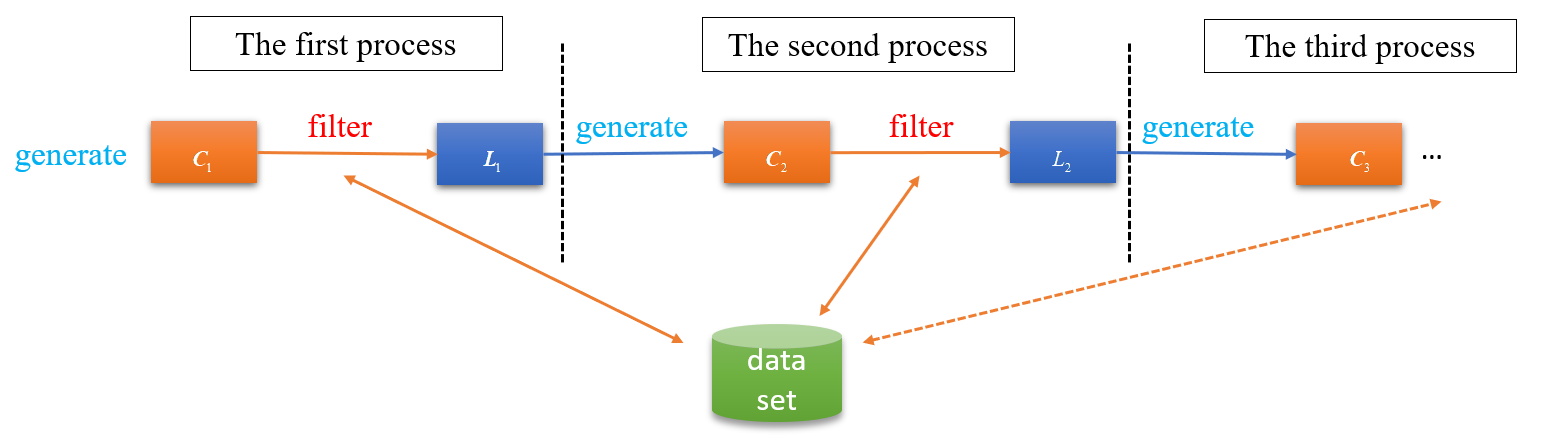
\includegraphics[scale=0.35]{9.1.1}
    \captionof{figure}{Apriori algorithm schematic diagram}
    \label{fig:9.1.1}
    \end{minipage}
    \par
    Before using the Apriori algorithm, you need to introduce concepts such as association rules, support, and confidence. Let $X={x_1 ,x_2 ,\dots,x_n}$, let A and B be itemsets, and the association rule $A\subset B$ is satisfied, A and B are disjoint. The definition of support is as follows:
    \begin{equation}
    \operatorname{support}(A B)=P(A \cup B)=\frac{\frac{D_{A} \rightarrow B}{D} \times 100 \%}{D}
    \end{equation}
    \par
    D represents the total amount of data, while $\mathrm{N}=\mathrm{A} \cup \mathrm{B}$ is the amount of data containing both A and B, meaning the proportion of data covered by the association rule, that is, the probability of A and B appearing in the total amount of data at the same time.
    \par
    The definition of confidence is as follows:
    \begin{equation}
    \text { confidence }(A B)=P(B \mid A)=\frac{D_{A} \rightarrow B}{D_{A}} \times 100 \%
    \end{equation}
    \par
    $D_{A}$ is the amount of data in A, the probability that the amount of data that contains item set A also contains item set B.
    \par
    A strong rule is defined to be greater than both the support threshold (min\_suppt) and confidence threshold (min\_conf). Item sets are called item sets, k-item sets are items containing K items, and frequent K-item sets are denoted as $L_k$.
    \par
    \textbf{In this case, perform the following steps:}
    \subparagraph{1}
    One-hot encoding of data.
    \subparagraph{2}
    Define association rules, support, and confidence.
    \subparagraph{3}
    Mining association rules using Apriori.
    \subparagraph{4}
    Calculate the specific review words that are most relevant to each star class.
    \subsection{Results and Analysis}
    In the case of hair\_dryer, high ratings are strongly associated with "love", "great", etc. while low ratings are often accompanied by "cost", "heavy". From the strong association rules of the three products, it is found that the higher the star rating, the specific review words tend to be common praise words or praise words of the product. The lower the star rating is, the specific comments are basically bad comments. Some comments directly point out the problems of the product. This kind of bad comments is an important way to improve sales strategy and understand the shortcomings of the product.
    \section{Model Analysis}
    \subsection{Strengths and Weaknesses}
    \paragraph{Strengths}
    \begin{enumerate}
        \item LDA topic model can analyze text and extract topics well.
        \item Combined EWM and TOPSIS, comprehensively evaluated the reputation rate of the product by taking full consideration of various indicators, which effectively solved the one-sidedness of the single index of star rating, help rate and satisfaction rate.
        \item Creatively propose normal and abnormal products, use OneClassSVM to get abnormal products, and then distinguish potential successful or failed products.
        \item Apriori algorithm can effectively help us obtain the association between specific review words and stars.
    \end{enumerate}
    \paragraph{Weakness}
    \begin{enumerate}
        \item Topics extracted by LDA are not necessarily valid.
        \item The results of Apriori algorithm need to be selected manually, and the required results cannot be given according to the needs.
    \end{enumerate}
    \subsection{Sensitivity Analysis}
    There are two hyperparameters in the LDA model, $\eta$ and $\alpha$ the hyperparameter representing the topic distribution and the document topic distribution respectively. And based on the following joint probability density:
    \begin{equation}
    p(\theta, \beta, w, z \mid \eta, a)=\prod_{-1}^{D} p(\theta, \mid \alpha) \prod_{\mid=1}^{C} p\left(\beta_{1} \mid \eta\right) \prod_{-1}^{N_{H}} p\left(w_{j, n} \mid z_{2, n}, \beta_{2}\right) p\left(z_{j, n} \mid \theta_{j}\right)
    \end{equation}
    \par
    When $\eta$ and $\alpha$ is changed, that is, when conditions in conditional probability are changed, the joint probability will change and the solution result will also change. We adjust the original $\eta$=0.6 and $\alpha$=0.3 to $\eta$=0.4 and $\alpha$=0.7 to observe whether the topic extracted from comments has changed significantly, and take satisfaction rate of comments as the judgment standard. Take the comments in the hair\_dryer section as an example, the results are shown in the following Table~\ref{tab:10.1.1}:\\[1em]
    \begin{minipage}{1.0\linewidth}
    \captionof{table}{Comment subject sensitivity analysis}
    \label{tab:10.1.1}
    \begin{threeparttable}[b]
    	\begin{tblr}{
          width=\linewidth,
          colspec={*{7}{X[c]}},
          hline{1, Z} = {2pt, solid},
          hline{2} = {solid}
        }
        review\_id & … & star\_rating & helpful\_ratio & S & s\_new & rate of change\\
        R230LCPQDOFJJZ & … & 5 & 0.5 & 0.87 & 0.84 & D 3.45\%\\
        R21NN9ONVZITI0 & … & 1 & 0.5 & 0.79 & 0.75 & D 2.53\%\\
        … & … & … & … & … & … & … \\
        R3N0F2FKJOMGKK & … & 5 & 0.95 & 0.95 & 0.96 & I 1.05\%
        \end{tblr}
        \begin{tablenotes}[flushleft]
        	\item Note: We use I for increase and D for decrease.
        \end{tablenotes}
    \end{threeparttable}
    \end{minipage}
    \par
    It is not difficult to find that the satisfaction rate of comments does not increase or decrease significantly and the change rate is small, indicating that the model is insensitive to the change of hyperparameters and the model has good robustness.
    \section{Conclusion}
    E-commerce platforms led by Amazon have been integrated into our lives. In order to help Sunshine Company prepare for online sales, we combined data analysis with LDA model to analyze the characteristics of data. Secondly, we built a self-built corpus to construct classic example sentences, analyzed them with Word2vec, and then clustered the comments into four categories: Good, good, poor and very poor, corresponding to grades 1, 2, 3 and 4, respectively. Then, EWM-Topsis is used to obtain reputation R, ARIMA is used to predict the increase and decrease of R, and the trend can be obtained by observing the sequence diagram. SVM was used to distinguish between successful and unsuccessful products using reputation as a criterion. In addition, we also use the Apriori algorithm, mining strong association rules, to get three products of high and low star corresponding specific comment words, such as hair\_dryer, high star with "love", "great", low star with "cost", "heavy" and so on. Finally, write to the director of Sunshine company with advice on "focusing on bad reviews and improving quality".
    \section{Letter}
    \noindent{}Dear Sunshine Company Marketing Director:
    \par
    We are honored to present to you our team's data analysis and results, and to give you sound recommendations for your three products.
    \par
    The first step is data preprocessing. The comments with VINE N and verified\_purchase N are rejected. Step 2: Data visualization, visualize the review stars and construct helpful\_ratio using the sigmoid function. Step 3: Descriptive statistics, descriptive statistics of review stars and Helpful\_ratio. Then the LDA topic model is constructed to extract the topic of each comment. It was found that the effect was very good after data cleaning, and there were almost no comments with a help rate lower than 0.5. Five-star reviews were always the most among the three products, and the distribution of five-star reviews was roughly the same between pacifier and Hair\_dryer, while the two-star reviews were the least, indicating that the quality of the two products was generally satisfactory, but still needed to be strengthened. However, the number of one-star reviews in microwave is second only to that of five-star reviews, indicating that there may be quality problems and other aspects, so we need to pay attention to the specific content of one-star reviews.
    \par
    Then, by using effective review subject, considering the need structure similarity, need self-built corpus, this can comment on the best use of existing information, on this basis to build five classic example, set up corresponding score of 0.1, 0.3, 0.5, 0.7, 0.9, use Word2vec to comment and classic example similarity analysis, The satisfaction rate of each comment is defined as the product of the score of the classic example with the greatest similarity and the maximum similarity. Then combining satisfaction rate, star rating and helpful\_ratio, k-means algorithm is used to classify customers' comments on products, so as to obtain valuable comments. Customers' comments on products are divided into four categories: Reviews in the "very good" category reveal the advantages of a product, while reviews in the "very bad" category are often the most valuable, and are key to improving a product and influencing decision making.
    \par
    In addition, in order to reflect the increase or decrease of product reputation, we defined the reputation rate R, completed the construction of the evaluation model of R through EWM-Topsis model, and took the final score as R. Since the data has date data every day, and Sunshine company also attaches great importance to time measurement, product review data can be regarded as a time series, and a prediction model of product reputation rate is constructed through ARIMA model to quantitatively analyze whether reputation is increasing or decreasing. Moreover, in order to define the evaluation criteria of potential success or failure, we first used One Class SVM model to distinguish normal products from abnormal products (potential success or failure products), and then trained SVM model to give judgment of successful or failed products, and achieved good results.
    \par
    Finally, we discuss the correlation between review stars and reviews and find strong association rules between review stars and specific review words. We first use Pearson correlation coefficient to explore the correlation between stars and the number of reviews, as well as between stars and review levels. It is found that the higher the star\_rating is, the more reviews there are, and the more favorable reviews there are; the lower the star\_rating is, the fewer reviews there are, and the more negative reviews there are. In order to find strong association rules, we used Apriori algorithm and found that for hair dryers, high stars often correspond to "hot" and "Quick", while low stars often correspond to "waste money". Therefore, hair dryers should be hot enough to dry hair quickly, but not too expensive. For pacifiers, high stars tend to correspond to "clean" and "soft", while low stars tend to correspond to "hard" and "small". Therefore, baby pacifiers should be soft, the right size and fit the baby. For a microwave oven, a high star usually corresponds to easy or fit, while a low star usually corresponds to Repair. Therefore, microwave ovens should be easy to use and provide excellent after-sales service.
    \par
    The above is our team's analysis results and suggestions for you. We sincerely hope that our research results and suggestions can help your products succeed. Looking forward to your reply, thank you!
    \par
    {\hfill Sincerely}
    \par
    {\hfill Team 2019057552}
\end{document}
%%% Local Variables:
%%% mode: latex
%%% TeX-master: "../mcmpaper"
%%% End:
